\documentclass[oneside,10pt,a4paper]{report}
\usepackage[a4paper, left=3cm, right=3cm, top=3cm, bottom=3cm, headsep=10mm, footskip=12mm]{geometry}
\usepackage[T1]{fontenc}
\usepackage[ngerman, english]{babel}    % mehrsprachiger Textsatz
% babel: letzte Sprache in Optionen zeigt die Sprache des Dokumentes
% und kann durch den Befehl \selectlanguage{} geaendert werden
% Passen Sie die Optionen des babel-Paketes nach Bedarf an!
\usepackage{float}
\usepackage{graphicx}
\usepackage{url}
\usepackage{pdflscape}
\usepackage{mathtools}
\usepackage{amssymb, amsmath, amstext}
\usepackage{amsthm}
\usepackage{xcolor}
\usepackage{nameref}
\usepackage{siunitx}
\usepackage{makecell}
\usepackage{hyperref}
\usepackage{enumitem}
\usepackage[superscript,biblabel]{cite}
\usepackage{caption}
\usepackage{subcaption}
\usepackage{tabularx} 			% Tabellen erzeugen
\usepackage{multirow}			 % Zeilen in Tabellenbearbeitung
\usepackage{multicol} 			% Spalten in Tabellenbearbeitung 
\usepackage{lmodern}                        % Ersatz fuer Computer Modern-Schriften 
\usepackage{amsmath}                                           % zum besseren Aussehen am Bildschirm
\usepackage{booktabs} % für schönere Tabellen
\usepackage{sidecap}
\usepackage{rotating} % für die Landscape-Umgebung
\usepackage{afterpage}
\definecolor{Bluetitle}{HTML}{1F3864}
\definecolor{softbluetitle}{HTML}{274D7E}
\definecolor{Greyish}{HTML}{5A5A5A}
%\renewcommand{\refname}{Reference}
\usepackage{array,multirow}
\newcommand{\specialcell}[2][c]{%
	\begin{tabular}[#1]{@{}c@{}}#2\end{tabular}}
\usepackage{titlesec}

\titleformat{\chapter}[display]
{\normalfont\bfseries}{}{0pt}{\Huge}

\usepackage{lipsum} 


\begin{document}
	
	\begin{titlepage}
		
		
	
		
		\begin{center}
			\begin{figure}[h!tbp]
				
\includegraphics[width=\linewidth]{HUlogo.PNG}
			\end{figure}
		\end{center}
			
			
			\textcolor{Greyish}{\textbf{Lebenswissenschaftliche Fakultät}}\par
			\textcolor{Greyish}{Institut für Biologie}\par
			\textcolor{Greyish}{Institute for Theoretical Biology)}\par
			\vspace*{4 cm}
		\begin{center}
			
			\textcolor{softbluetitle}{\textbf{\Large Studienprojekt}}\par
			\vspace*{1 cm}
			\textcolor{Bluetitle}{\textbf{\Huge Implementing ODE Models for Biological Oscillators}}\par
			\vspace*{1 cm}
			\textcolor{softbluetitle}{\textbf{\Large Coupling Duffing and Van der Pol Oscillators}}\par
			
		\end{center}
			\vspace*{4cm}
		
			
			
			\vspace*{0.5cm}
			\textcolor{Greyish}{vorgelegt von}\par
			\vspace*{0.5cm}
			\textcolor{Greyish}{Huyen Anh Nguyen}\par
			\textcolor{Greyish}{Matrikelnummer 572309}\par
			\textcolor{Greyish}{huyen.anh.nguyen@student.hu-berlin.de}\par
			\textcolor{Greyish}{Geboren am 14.03.1996 in Strausberg}\par
			\vspace*{0.5cm}
			\textcolor{Greyish}{Erstprüfer:		Prof. Dr. Hanspeter Herzel}\par
			\textcolor{Greyish}{Zweitprüfer:		Dr. Mathias König}\par
			
			
			
	
	\end{titlepage}
	
	
	\tableofcontents
	\chapter{Motivation}
	
		Many people enjoy listening to music. And in the music scene, there are many genres from classical music to heavy metal music. Fascinating tones are produced daily, which we can perceive with our ears and process in our brains. The tones are transmitted as sound waves to our ears through air, water, or solids and are generated by various sound wave producers, such as the vocal folds.\\
		We can perceive and produce both linear and nonlinear phenomena. \\
		Especially the nonlinear phenomena are particularly interesting, not only how we can produced them, but also the mathematical background of it is interesting.\\
		 For example, the metal singer Daniel Priegnitz can produce linear oscillatory movement sounds with his vocal folds driven by subglottic pressure, but he can also produce nonlinear sounds using well-known metal vocal techniques like "growling" with his false vocal folds (also called ventricular folds) \cite{DanielPriegnitz}.
		 Driven by the skills of Daniel Priegnitz and the desire to understand nonlinear sound production, two oscillator models (the Duffing oscillator and the Van der Pol oscillator) are implemented into one oscillator model. Each oscillator contributes its own properties to this new system.\\
		 In this short "Studienproject," I will explain the equations of the two chosen models (Duffing oscillator and Van der Pol oscillator) and try to understand how the period T, frequency f, and angular frequency $\omega$ will change for the new driven oscillator model. I will also analyze the amplitude response of the Duffing oscillator.\\
		 Although there are plenty of existing different models, the hope of this new model is to gain new insights into complex nonlinear sound production.
		 
		 
	\chapter{Duffing- and Van der Pol Oscillator} \label{chapter: Duffing- and Van der Pol Oscillator}
	
		The Duffing and Van der Pol oscillators are both nonlinear oscillators, each with their own special properties. 
		The two oscillators will be described in the following sections as uncoupled, non-driven, autonomous oscillators.
		
		\section{Duffing-Oscillator}
		Wenn man einem linearen 2. Ordnung des mass-spring harmonic Oscillators-Ordinary Differential Equation (Abberation: ODE) einem nicht-linearen Term $\alpha y +\beta y^3$ hinzufügt, erhält man den Duffing-Oszillator\cite{twist_paper} ein nichtlineares System.
		
		\begin{equation}\label{eq: duffing_ungetrieben}
			\frac{d^2y}{dt^2} + \gamma \frac{dy}{dt} + \alpha y + \beta y^3 = 0
		\end{equation}
		Die folgenden Parameter der Gleichung \ref{eq: duffing_ungetrieben} sind in Table \ref{tab: duffing_ungetriebene_parameter} beschrieben und Werte ausgewählt. 
		
			\begin{table}[H]
			\centering
			\caption{The meaning of the Duffing Parameter and choosen values for them without units.}
			\label{tab: duffing_ungetriebene_parameter}
			\begin{tabular}{c c c}
				\toprule
				parameter & meaning & value\\
				\midrule
				$\gamma$ & damping term & 0.1\\
				$\alpha$ & linear restoring force & 0.1\\
				$\beta$& nonlinear restoring force & 0.2\cite{Parlitz_p93}\\
				\bottomrule
			\end{tabular}
		\end{table}
		
		In der Table \ref{tab: duffing_ungetriebene_parameter} wurden für $\beta$ > 0 den Wert nach Parlitz ausgewählt, somit besitzt das System hohe nicht-lineare Rückstellkraft und verhält sich weniger chaotisch und in den Ruhelage zurückkehrt. Für die anderen Parameter wurde für $\gamma$ < 1 gewählt, damit das System eine schwache Dämpfung widerfährt und für $\alpha$ < 1 nur eine kleine lineare Rückstellkraft hat, damit das System locker bleibt.
		
		
		\begin{figure}[H]
			\centering
			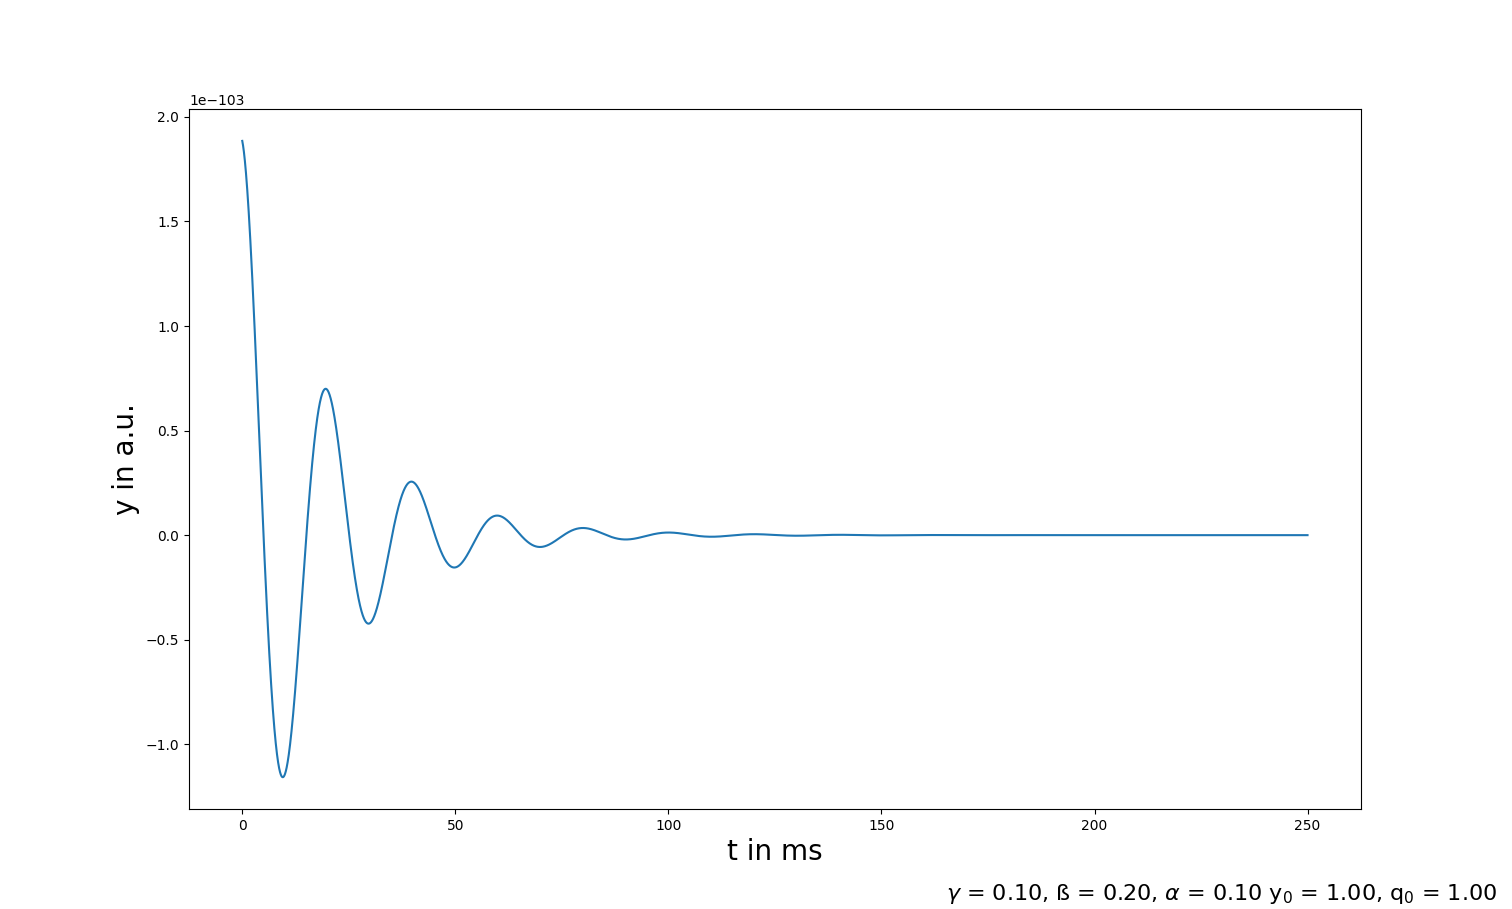
\includegraphics[scale=0.4]{duffing_unforced_y.png}
			\caption{Time curve of an unforced Duffing Oscillator with the parameter $\gamma$ = 0.1, $\alpha$ = 0.1 and $\beta$ = 0.2. The giving Startingpoint for this simulation is (y,p) = (1, 1) for t = [0,250] ms.}
			\label{fig: duffing_unforced_y}
		\end{figure}
		
		WIe man in Figure \ref{fig: duffing_unforced_y} sehen kann, kehrt das System schnell in seiner Ruhelage wieder zurück.
		
		\cite{Nonlinear_Dynamic_and_chaos_book}
	
		\section{Van der Pol - Oscillator}
		Auch der Van der Pol - Oscillator ist ein nonlinear System, wo ein harmonischen Oscillator ein nichtlinearen damping term $\mu$(x$^2$ - 1)$\dot{x}$ hinzugefügt wurde (siehe Gleichung \ref{eq: unforced_vdp}).
		
		\begin{equation}\label{eq: unforced_vdp}
			\frac{d^2x}{dt^2} - \mu (1 - x^2) \frac{dx}{dt} + x = 0
		\end{equation}
		
		Der Van der Pol Oszillator kann sich selbst erregen und in einen stabilen Grenzzyklus übergehen. 
		In Table \ref{tab: vdp_ungetriebene_parameter} wurde für $\mu$ = 0.1 gewählt, damit die nicht-lineare Dämpfung klein gehalten wird und das System sich ähnlich wie einen hramonischen Oszillator verhält, welches in Figure \ref*{fig: vdp_unforced_x} auch zu sehen ist.
			\begin{table}[H]
			\centering
			\caption{The meaning of the Duffing Parameter and choosen values for them without units.}
			\label{tab: vdp_ungetriebene_parameter}
			\begin{tabular}{c c c}
				\toprule
				parameter & meaning & value\\
				\midrule
				$\mu$ & damping term & 0.5\\
				\bottomrule
			\end{tabular}
		\end{table}
		
			\begin{figure}[H]
			\centering
			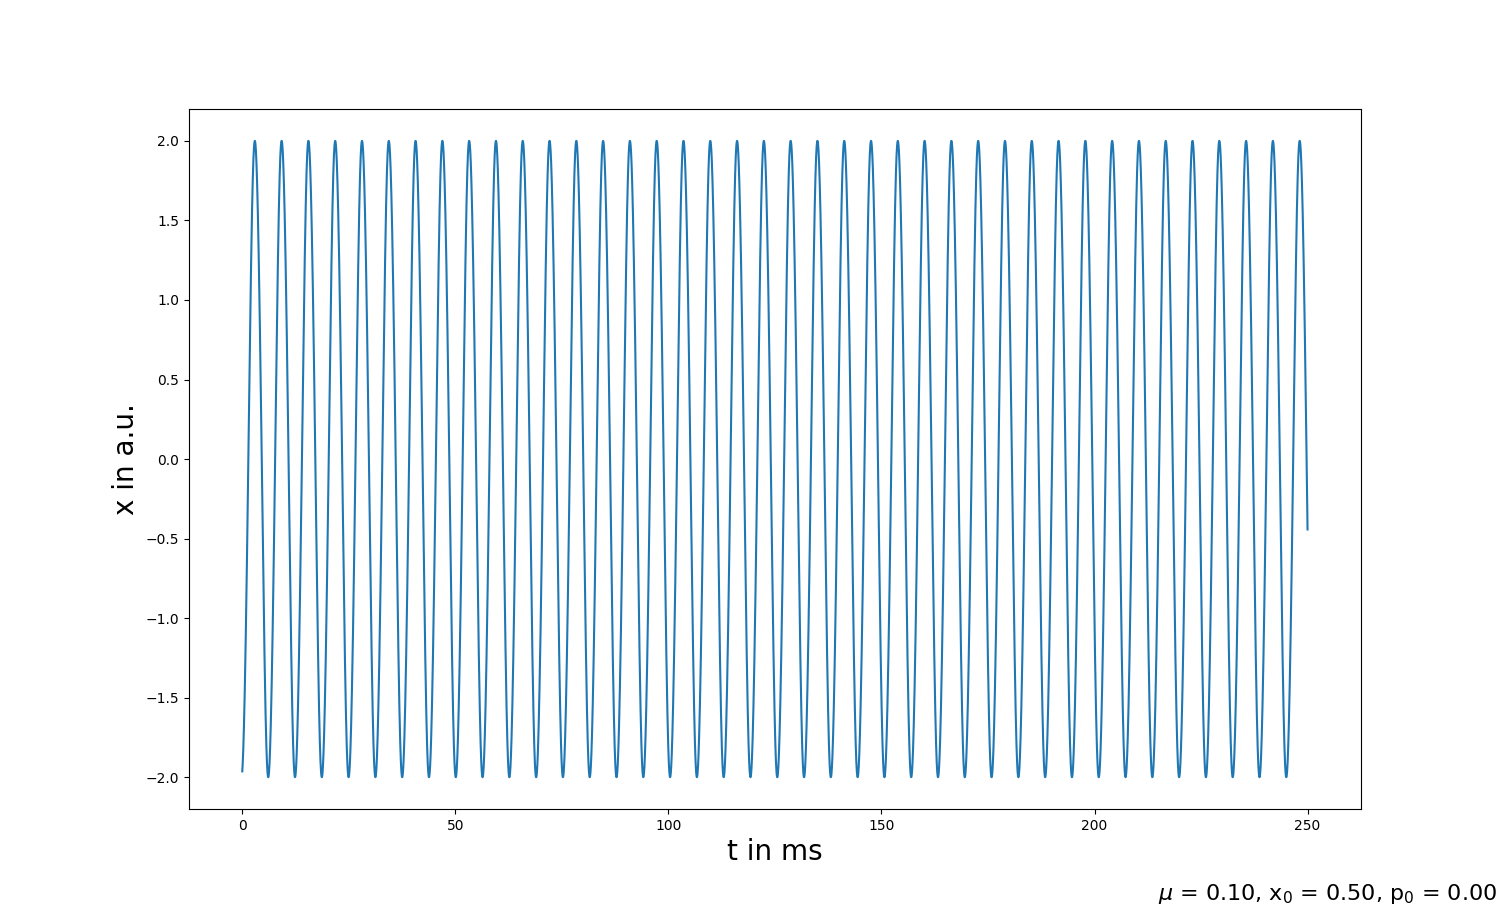
\includegraphics[scale=0.4]{vdp_unforced_x.png}
			\caption{Time curve of an unforced Van der Pol Oscillator with the parameter $\mu$ = 0.1, . The giving Startingpoint for this simulation is (x,q) = (0.5, 0)\cite{Nonlinear_Dynamic_and_chaos_book} for t = [0,250] ms.}
			\label{fig: vdp_unforced_x}
		\end{figure}
		
		\chapter{Implementing a new Oscillator-model}
		Im Chapter \ref{chapter: Duffing- and Van der Pol Oscillator} wurden die ungetrieben Oscillatoren vorgestellt. Was passiert aber, wenn man die Eigenschaften der beide autonomen Oscillatoren in einem neuen Differentialgleichung koppelt?
		Für den anfänglichen Implementierung wird der Duffing Oscillator (y(t)) mit den Van der Pol Oscillator (x(t)) additiv mit dem Kopplungsterm k gekoppelt (siehe Gleichung \ref{eq: vdp_duffing_ODE}).
		Dadurch treiben sich die beiden Oszillatoren und bilden ein nicht-autonomes System.
		\begin{equation}\label{eq: vdp_duffing_ODE}
			\begin{split}
				\frac{d^2x}{dt^2} - \mu (1 - x^2) \frac{dx}{dt} + x = k ( y- x )\\
				\frac{d^2y}{dt^2} + \gamma \frac{dy}{dt} + \alpha y + \beta y^3 = k ( x-y )\\
			\end{split}
		\end{equation}
		
		Die Lösung der gekoppelte ODE ist in Gleichung \refeq{eq: vdp_duffing_Lösung} dargestellt.

			\begin{equation}\label{eq: vdp_duffing_Lösung}		
			\begin{gathered}
				\frac{dx}{dt} = p\\
				\frac{dp}{dt} = \mu (1 - x^2) p - x +k ( y- x )\\
				\\
				\frac{dy}{dt} = q\\
				\frac{dq}{dt} = - \gamma q - \alpha y - \beta y^3 + k ( x-y )\\
			\end{gathered}		
		\end{equation}
		
		Für die Parameter wurden die Werte wie in Table \ref*{tab: duffing_ungetriebene_parameter} und \ref{tab: vdp_ungetriebene_parameter} beigehalten.\\
		Es wurde für k = 0.0, 0.01, 0.1, 0.5, 1.0 eine time serie numerisch integriert.\\
		Durch die Kopplung der beiden autonomen Oscillatoren verkleinert sich die Amplitude bei der Van der Pol - Oscillator bei wachsenden k und bei dem Duffing - Oscillator wächst die Amplitude.
		Es wurde mit Absicht nur für k < 1 simuliert, damit das chaotische Verhalten weitgehend minimiert wird. In der Table \ref{tab: freq_x} und \ref{tab: freq_y} wurde die Periode T, Frequency f, angular frequency $\omega$ und Amplitude A aus der Simulation in Figure \ref{fig: timekurve_k} bestimmt. Und da kann gesehen werden, dass bei den Van der Pol Oscillator die Werte sinken und bei den Duffing System die steigen, bei steigende k Wert.\\
		
		
		\begin{figure}[H]
			\centering
			\begin{subfigure}[b]{0.45\textwidth}
				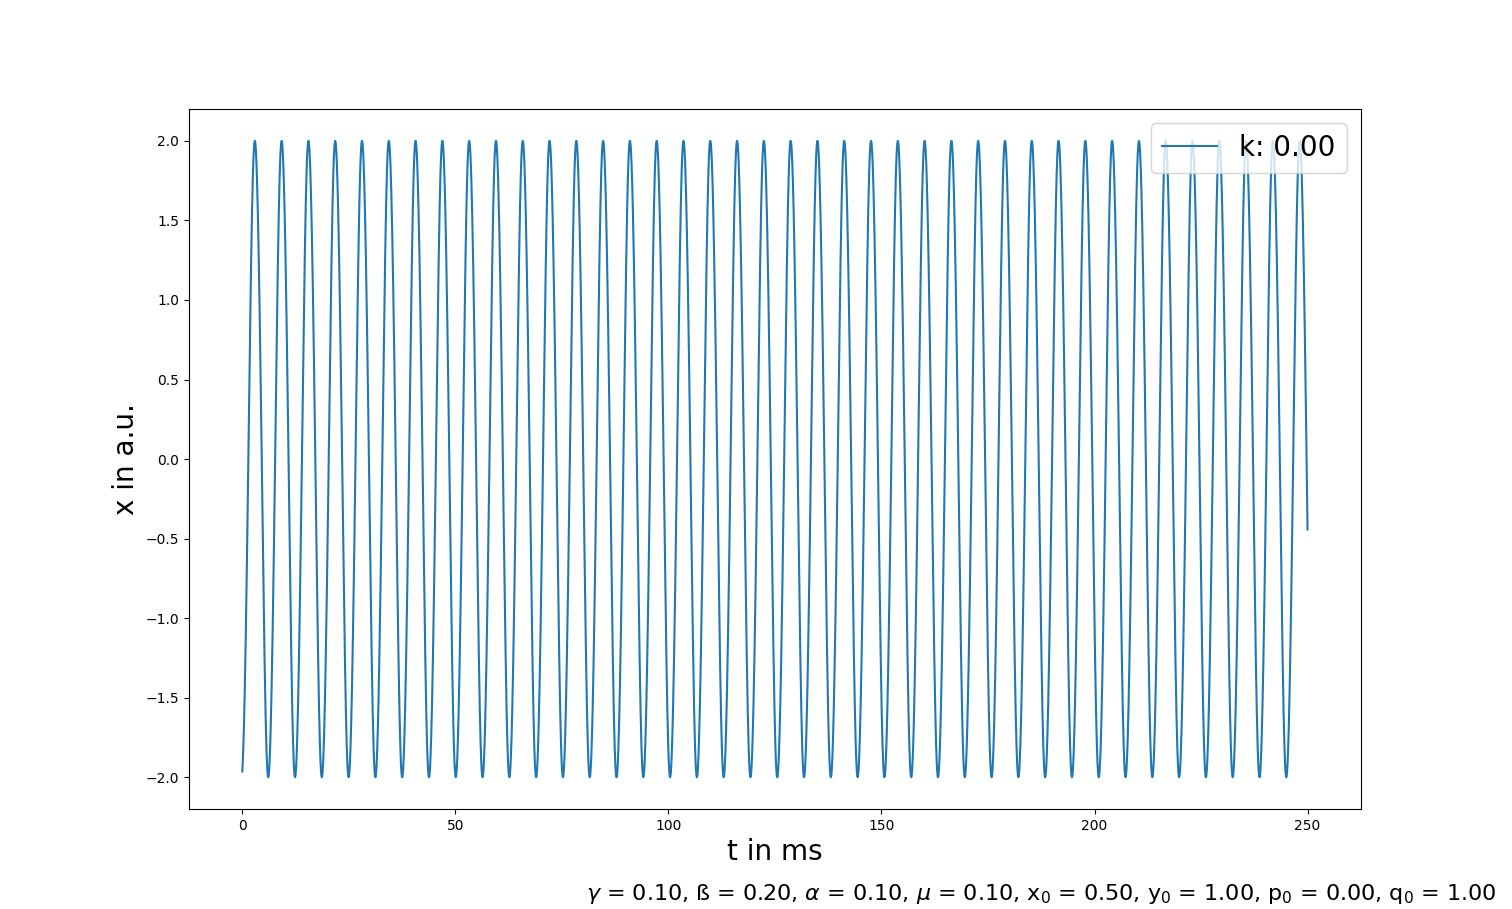
\includegraphics[width=\textwidth]{x_k1.png}
				\caption{}
				\label{fig:x1}
			\end{subfigure}
			\hfill
			\begin{subfigure}[b]{0.45\textwidth}
				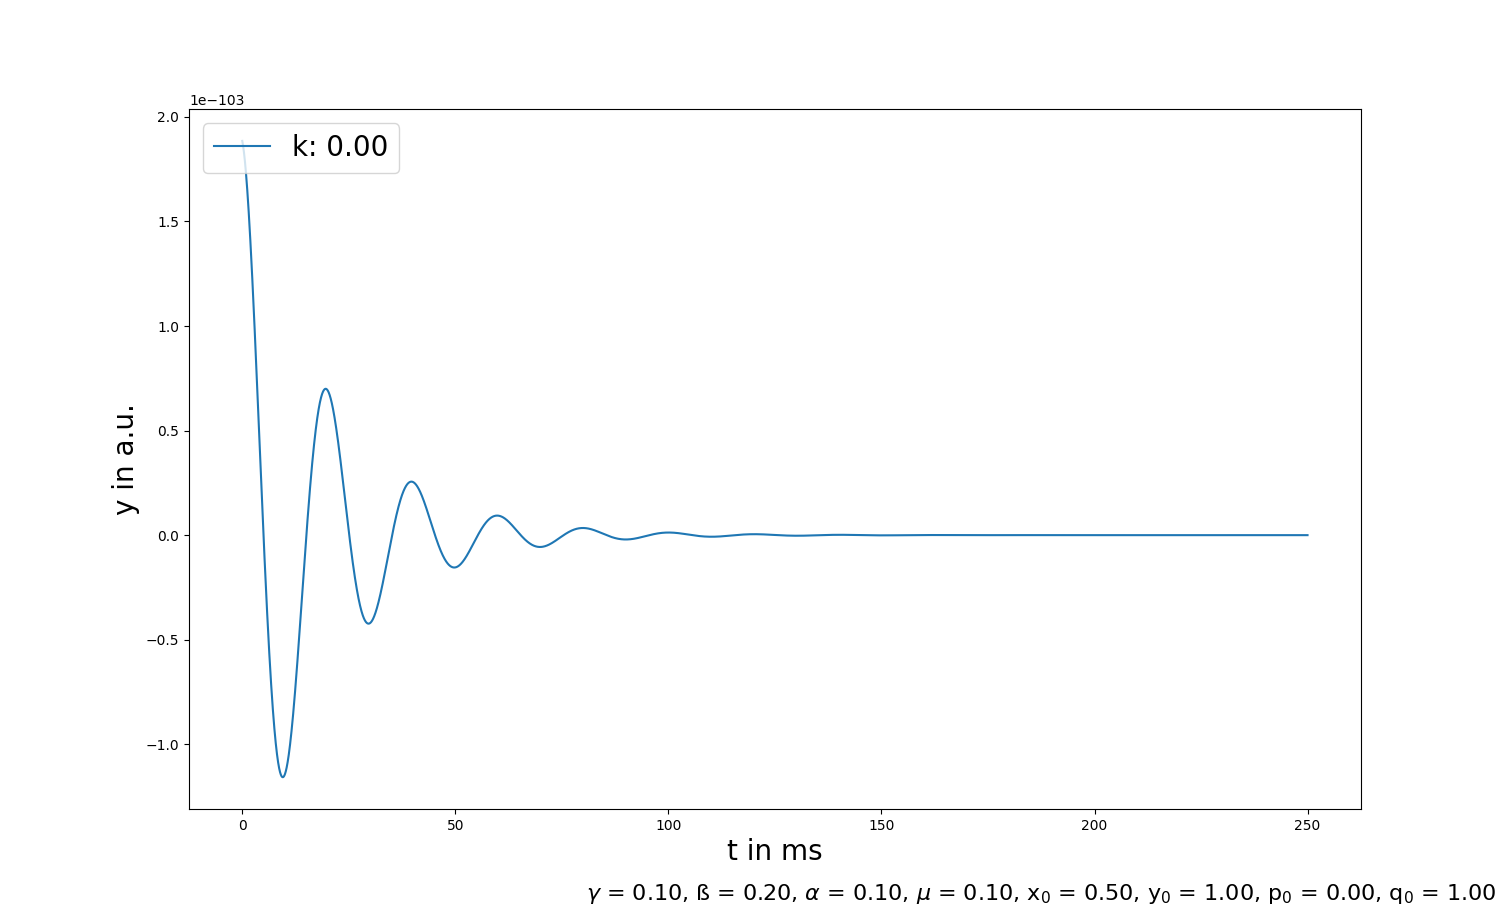
\includegraphics[width=\textwidth]{y_k1.png}
				\caption{}
				\label{fig: y1}
			\end{subfigure}
				\begin{subfigure}[b]{0.45\textwidth}
				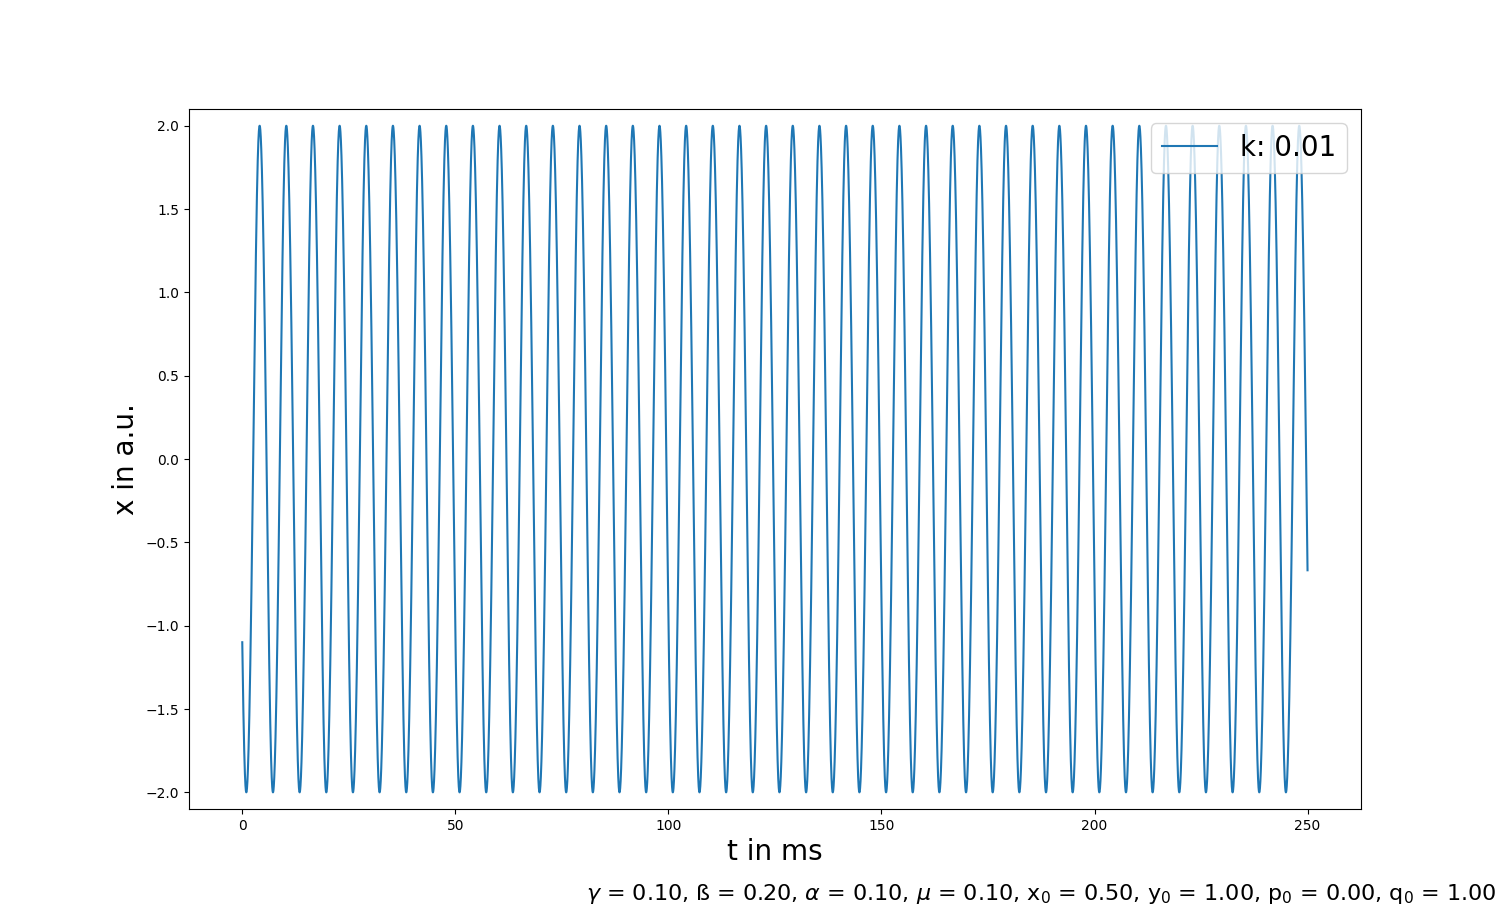
\includegraphics[width=\textwidth]{x_k5.png}
				\caption{}
				\label{fig:x5}
			\end{subfigure}
			\hfill
			\begin{subfigure}[b]{0.45\textwidth}
				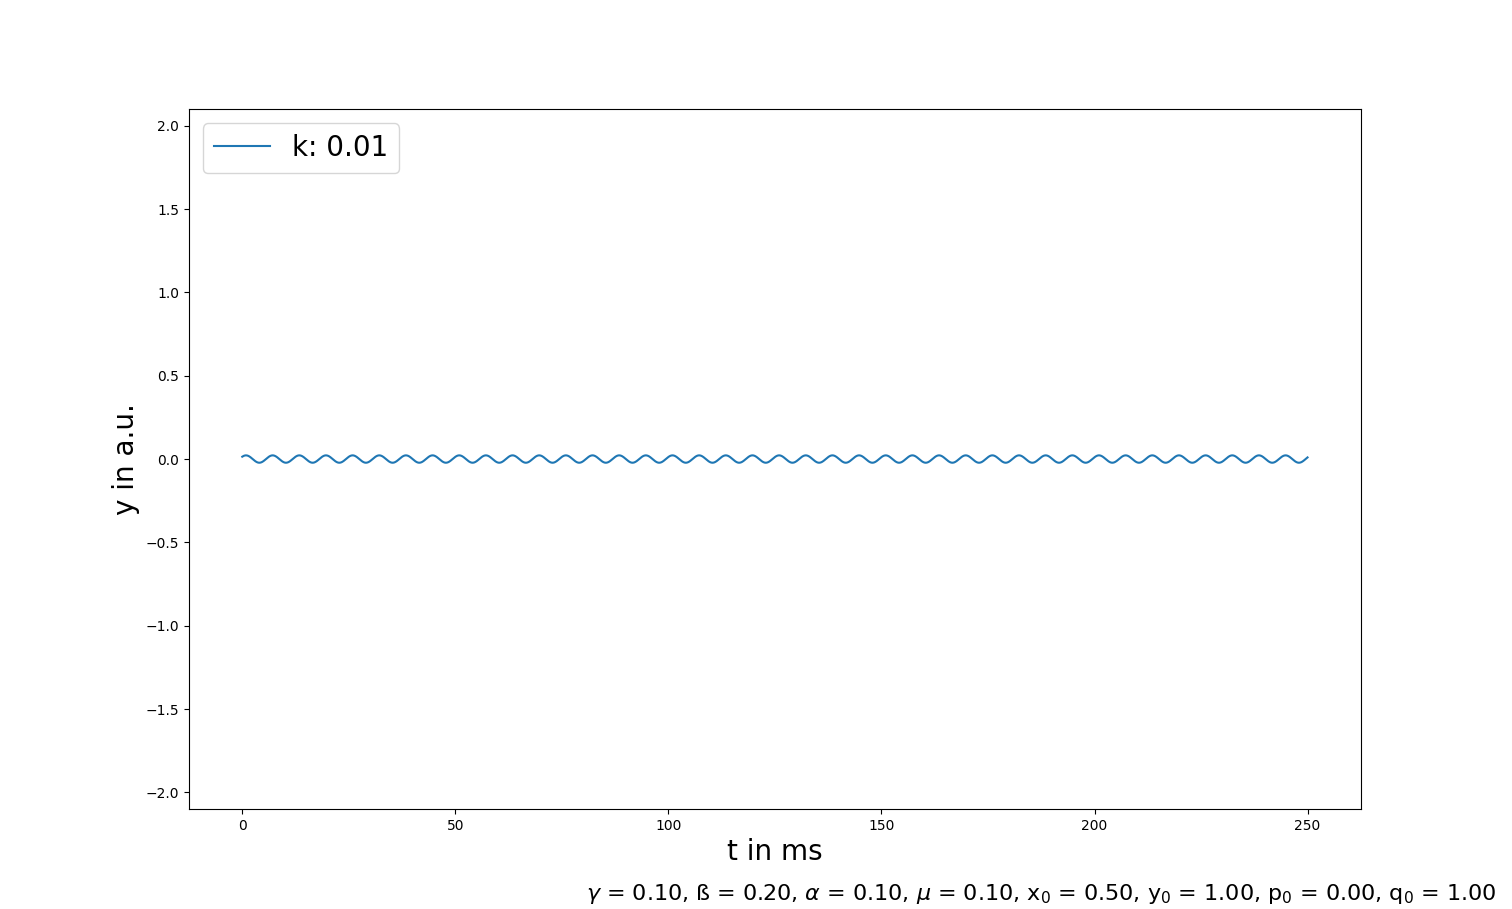
\includegraphics[width=\textwidth]{y_k5.png}
				\caption{}
				\label{fig: y5}
			\end{subfigure}
			\begin{subfigure}[b]{0.45\textwidth}
				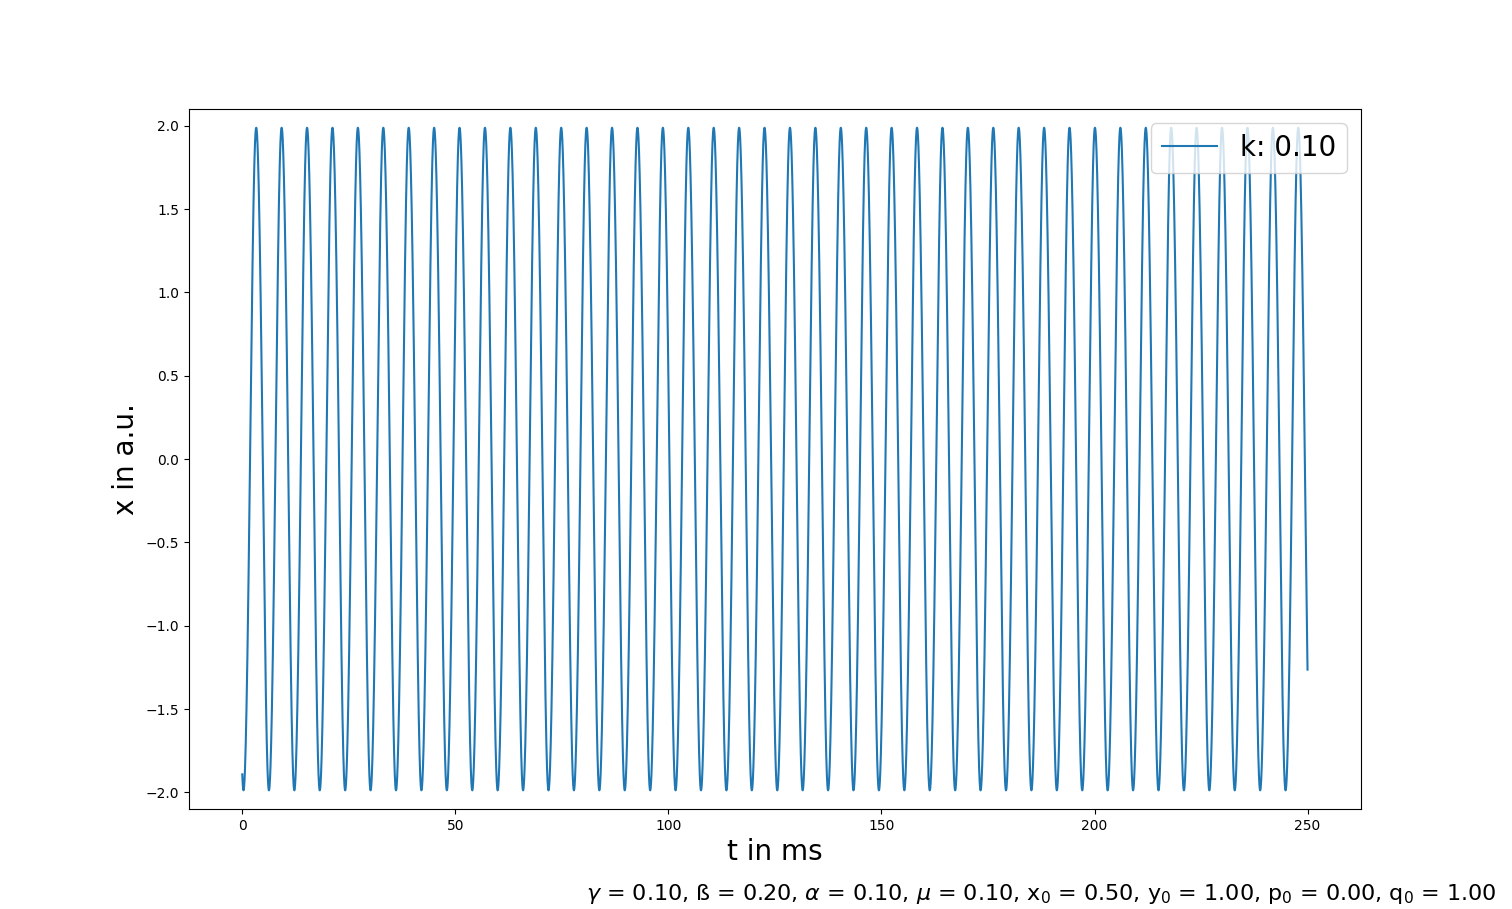
\includegraphics[width=\textwidth]{x_k2.png}
				\caption{}
				\label{fig:x2}
			\end{subfigure}
			\hfill
			\begin{subfigure}[b]{0.45\textwidth}
				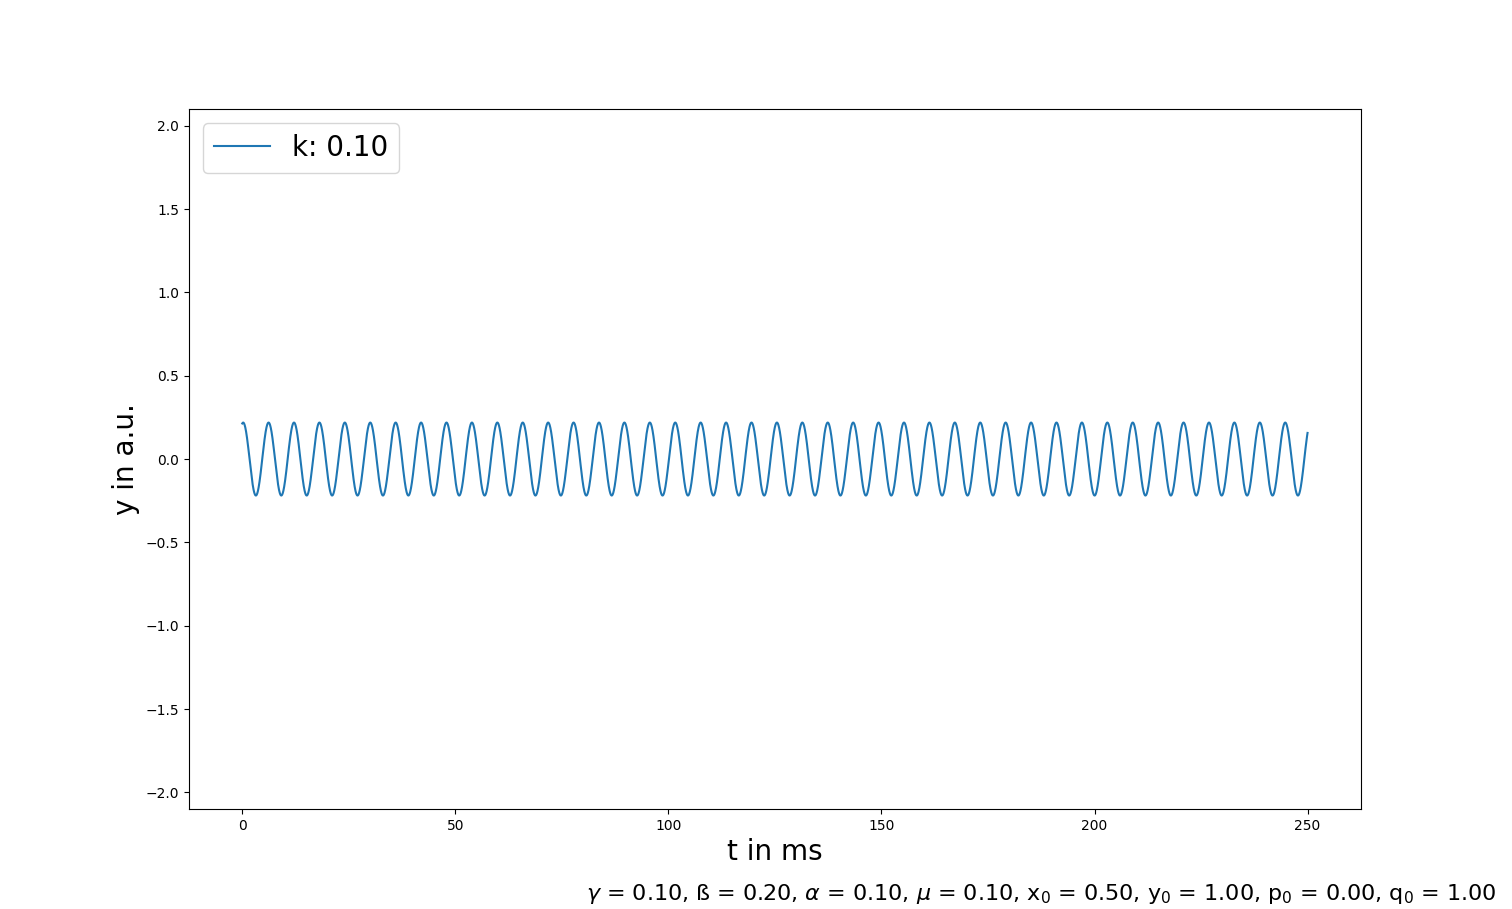
\includegraphics[width=\textwidth]{y_k2.png}
				\caption{}
				\label{fig: y2}
			\end{subfigure}
			\begin{subfigure}[b]{0.45\textwidth}
				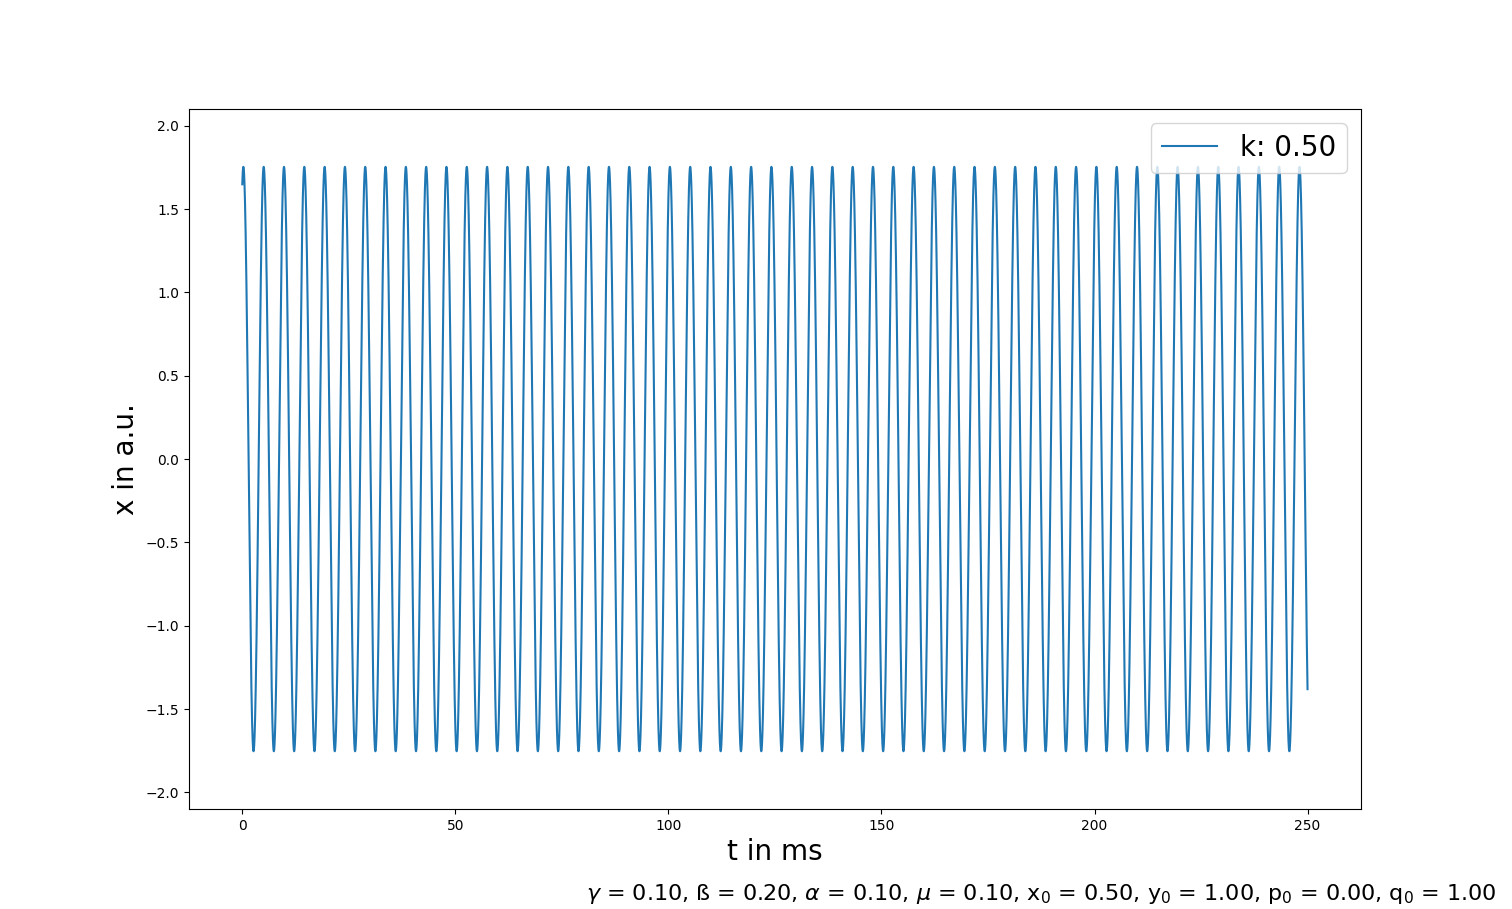
\includegraphics[width=\textwidth]{x_k3.png}
				\caption{}
				\label{fig:x3}
			\end{subfigure}
			\hfill
			\begin{subfigure}[b]{0.45\textwidth}
				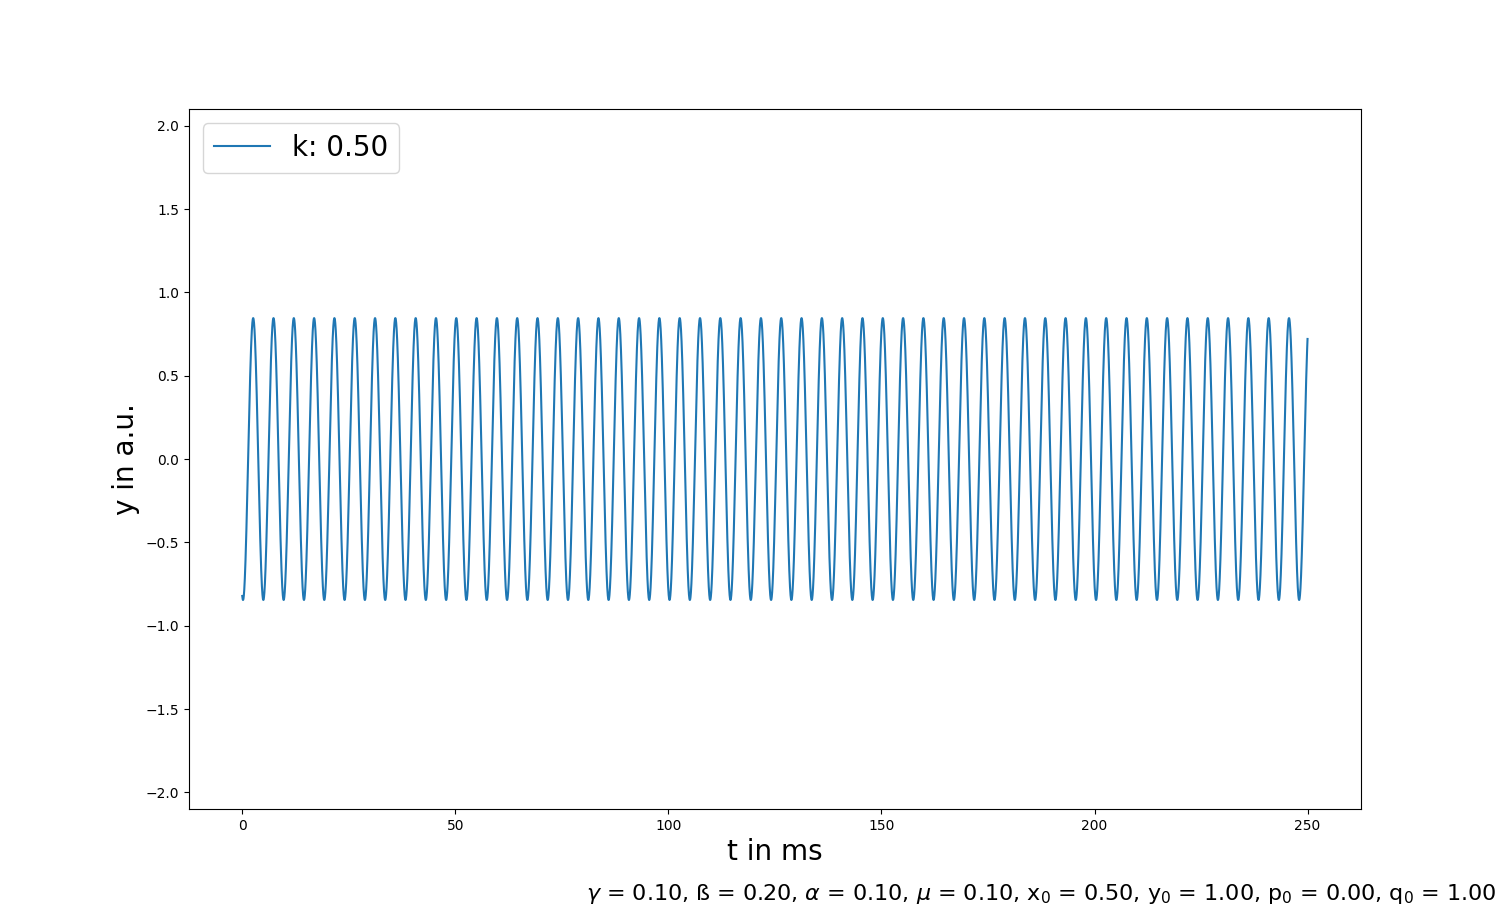
\includegraphics[width=\textwidth]{y_k3.png}
				\caption{}
				\label{fig: y3}
			\end{subfigure}
			\begin{subfigure}[b]{0.45\textwidth}
				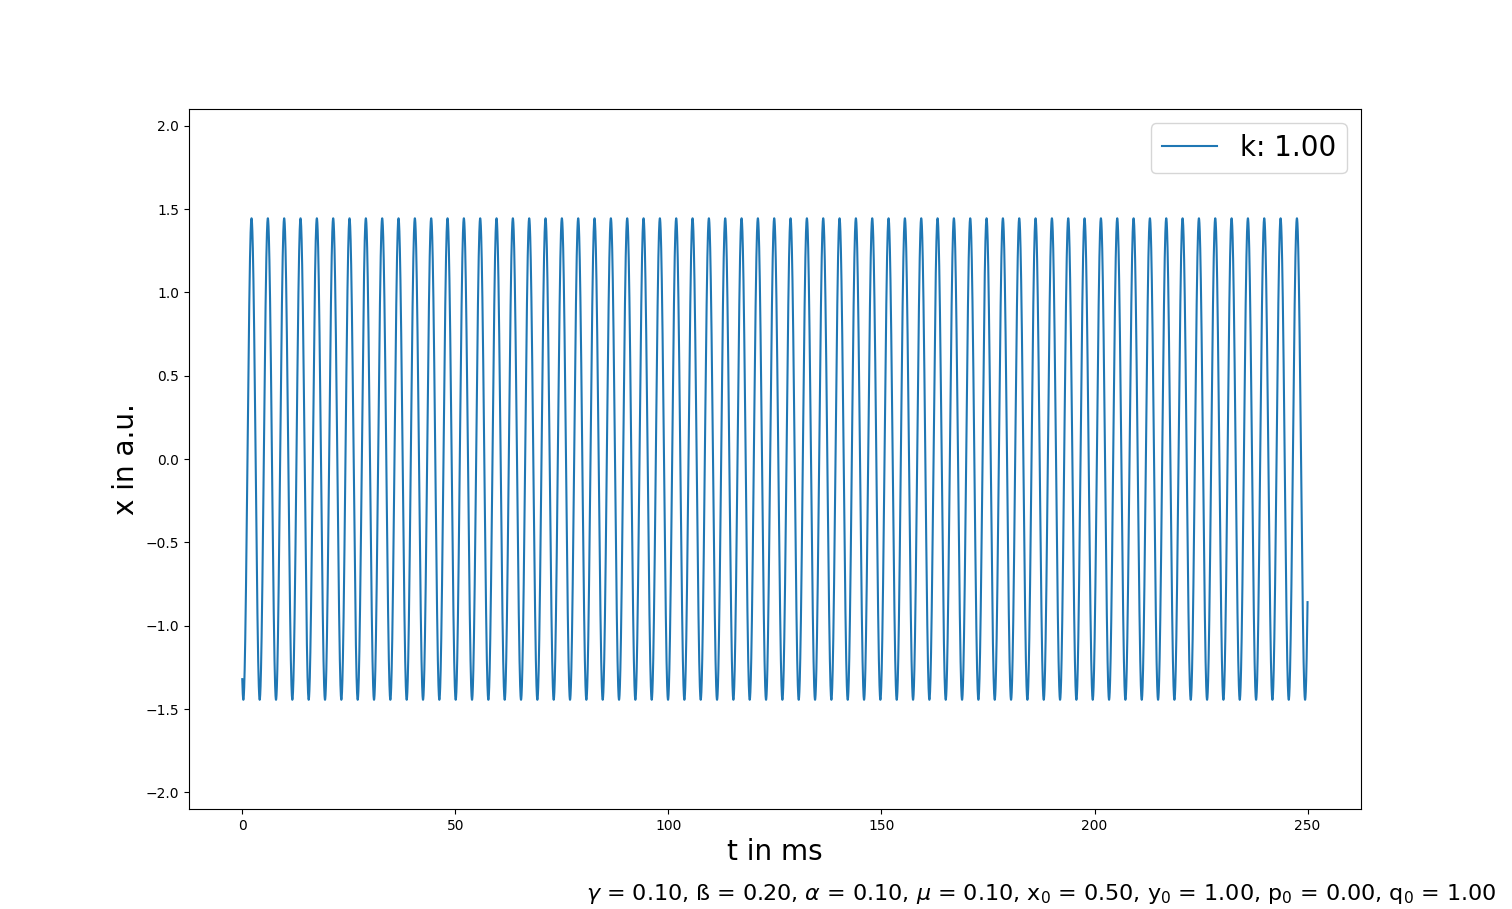
\includegraphics[width=\textwidth]{x_k4.png}
				\caption{}
				\label{fig:x4}
			\end{subfigure}
			\hfill
			\begin{subfigure}[b]{0.45\textwidth}
				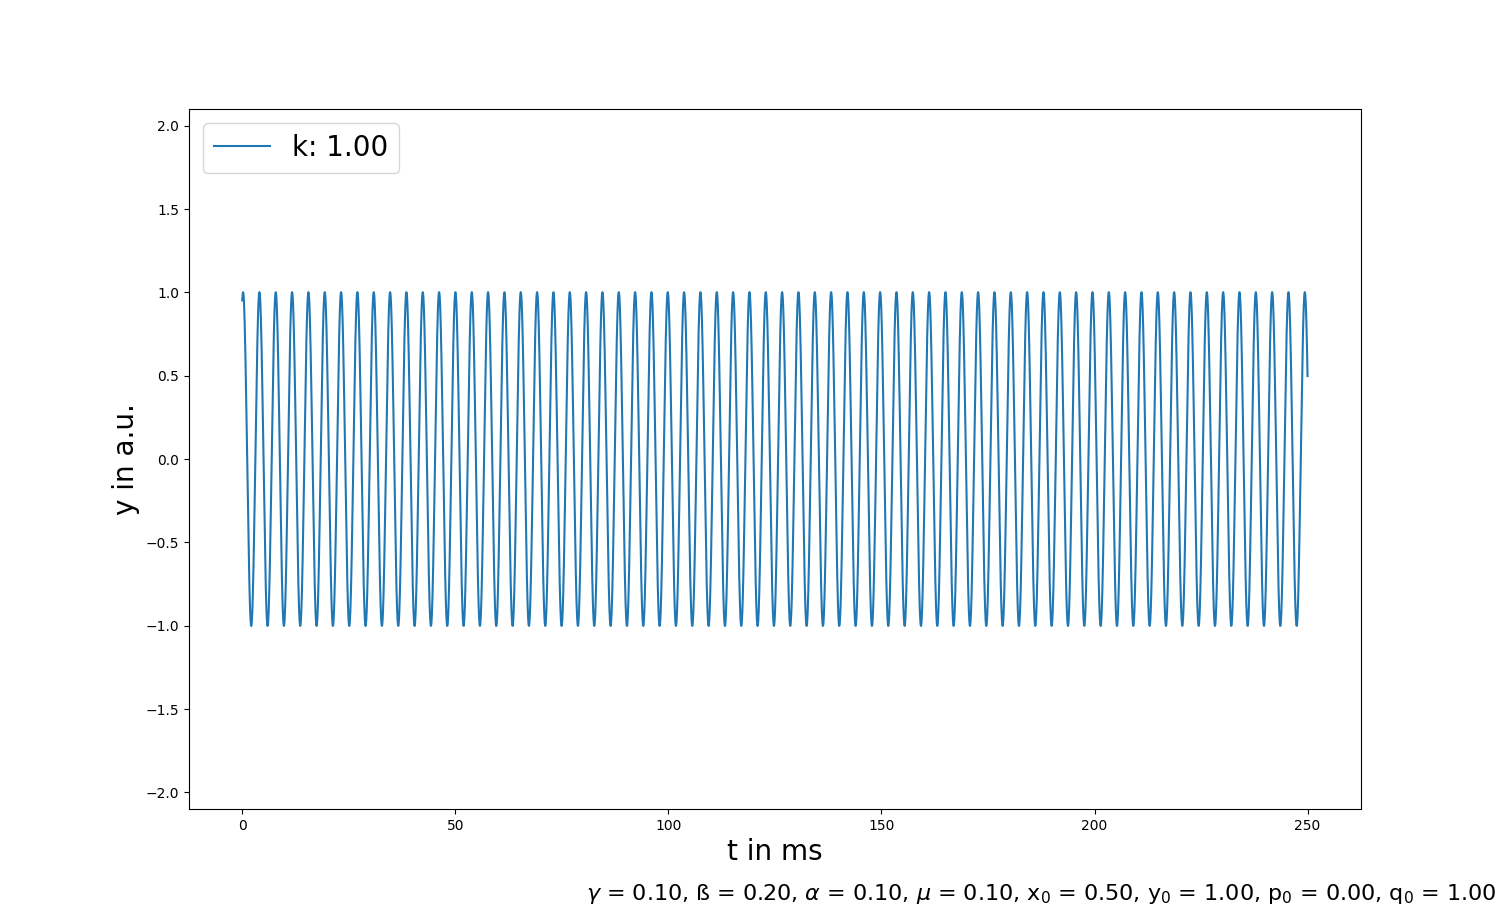
\includegraphics[width=\textwidth]{y_k4.png}
				\caption{}
				\label{fig: y4}
			\end{subfigure}
			\caption{Simulation of the additive coupled Duffing- Van der Pol - oscillators as a time series for t = [0, 250] ms. 
				Simulation of the model was with the following parameters: $\gamma$ = 0.1, $\alpha$ = 0.1 and $\beta$ = 0.2, $\mu$ = 0.1. The giving Startingpoint for this simulation is (x, q, y,p) = (0.5, 0.0, 1.0, 1.0).
				 (\ref{fig:x1}, \ref{fig: y1}) for k = 0.0, (\ref{fig:x5}, \ref{fig: y5}) for k = 0.01,(\ref{fig:x2}, \ref{fig: y2}) for k = 0.1, (\ref{fig:x3}, \ref{fig: y3}) for k = 0.5, (\ref{fig:x4}, \ref{fig: y4} ) for k = 1.0}
			\label{fig: timekurve_k}
		\end{figure}
		
		\begin{table}[H]
			\centering
			\caption{Additive coupled Van der Pol Oscillator x: Period T, Frequency f, angular frequency $\omega$ and Amplitude A for k = 0.00, 0.01, 0.10, 0.50, 1.00.}
			\label{tab: freq_x}
			\begin{tabular}{c c c c c}
				\toprule
				k & Period T & Frequency f & $\omega$ & Amplitude A \\
				\midrule
				0.00 & 6.29 & 0.16 & 1.00 & 2.00 \\
				0.01 & 6.26 & 0.16 & 1.00 & 1.99 \\
				0.10 & 5.96 & 0.17 & 1.05 & 1.98 \\
				0.50 & 4.79 & 0.21 & 1.31 & 1.71 \\
				1.00 & 3.90 & 0.26 & 1.61 & 1.37 \\
				\bottomrule
			\end{tabular}
		\end{table}
		\begin{table}[H]
			\centering
			\caption{Additive coupled Duffing Oscillator y: Period T, Frequency f, angular frequency $\omega$ and Amplitude A for k = 0.00, 0.01, 0.10, 0.50, 1.00.}
			\label{tab: freq_y}
			\begin{tabular}{c c c c c}
				\toprule
				k & Period T & Frequency f & $\omega$ & Amplitude A \\
				\midrule
				0.00 &19.92 & 0.05 & 0.32 & - \\
				0.01 & 6.38 & 0.16 & 0.98 & 0.03 \\
				0.10 & 6.01 & 0.17 & 1.05 & 0.23 \\
				0.50 & 4.80 & 0.21 & 1.31 & 0.84 \\
				1.00 & 3.92 & 0.26 & 1.60 & 0.96 \\
				\bottomrule
			\end{tabular}
		\end{table}
		
		Durch die Kopplung kann der Duffing-Oscillator seine Schwingung beibehalten. In 
	\begin{figure}[H]
		\centering
		\begin{subfigure}[b]{0.45\textwidth}
			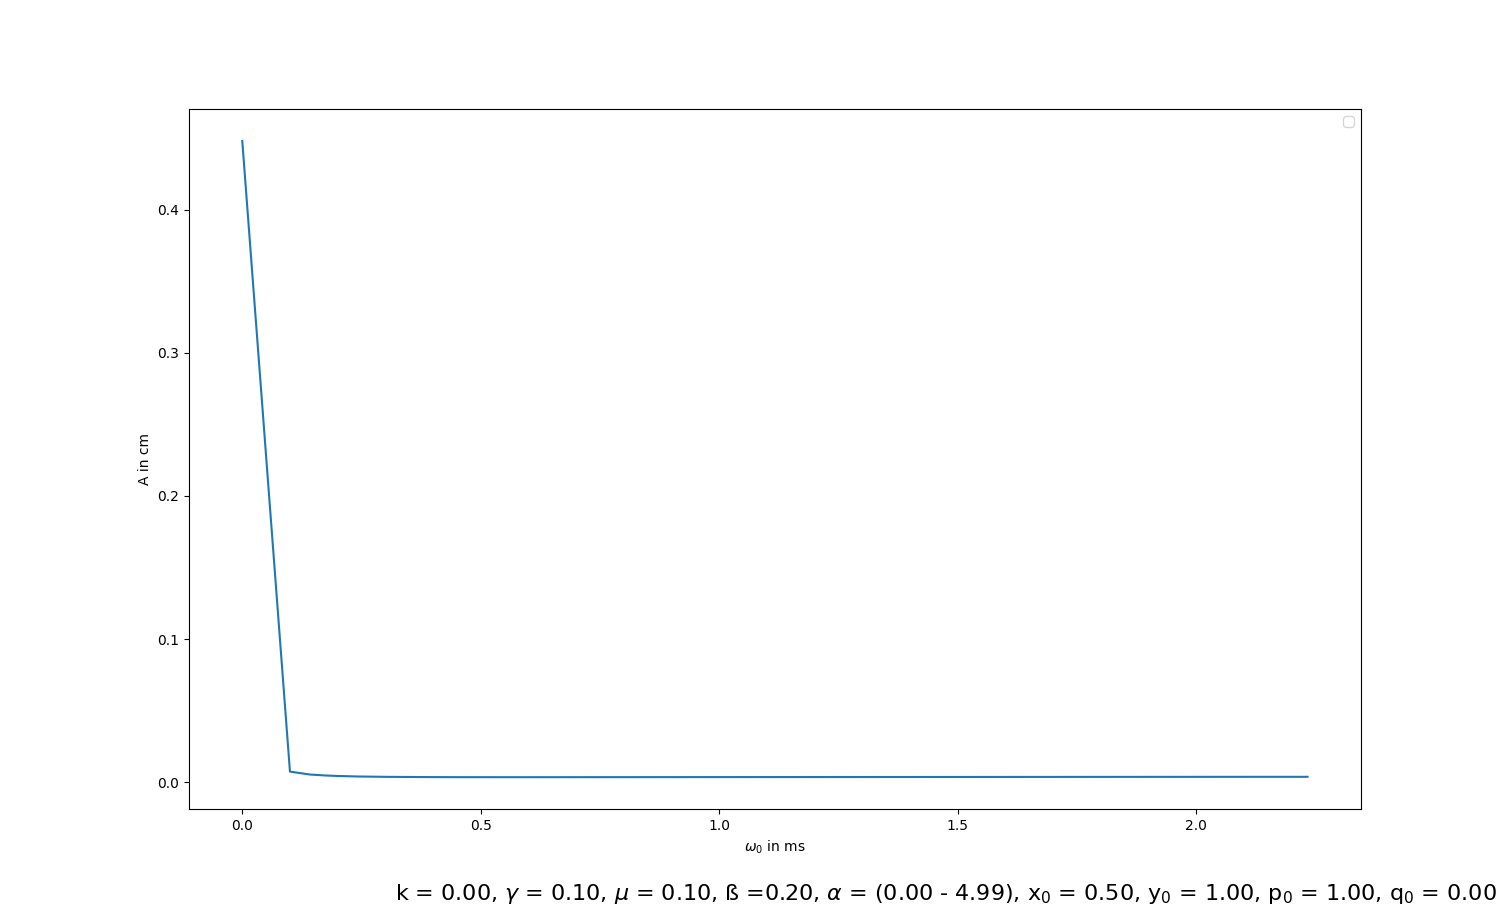
\includegraphics[width=\textwidth]{resonanz1.png}
			\caption{}
			\label{fig:resonanz1}
		\end{subfigure}
		\hfill
		\begin{subfigure}[b]{0.45\textwidth}
			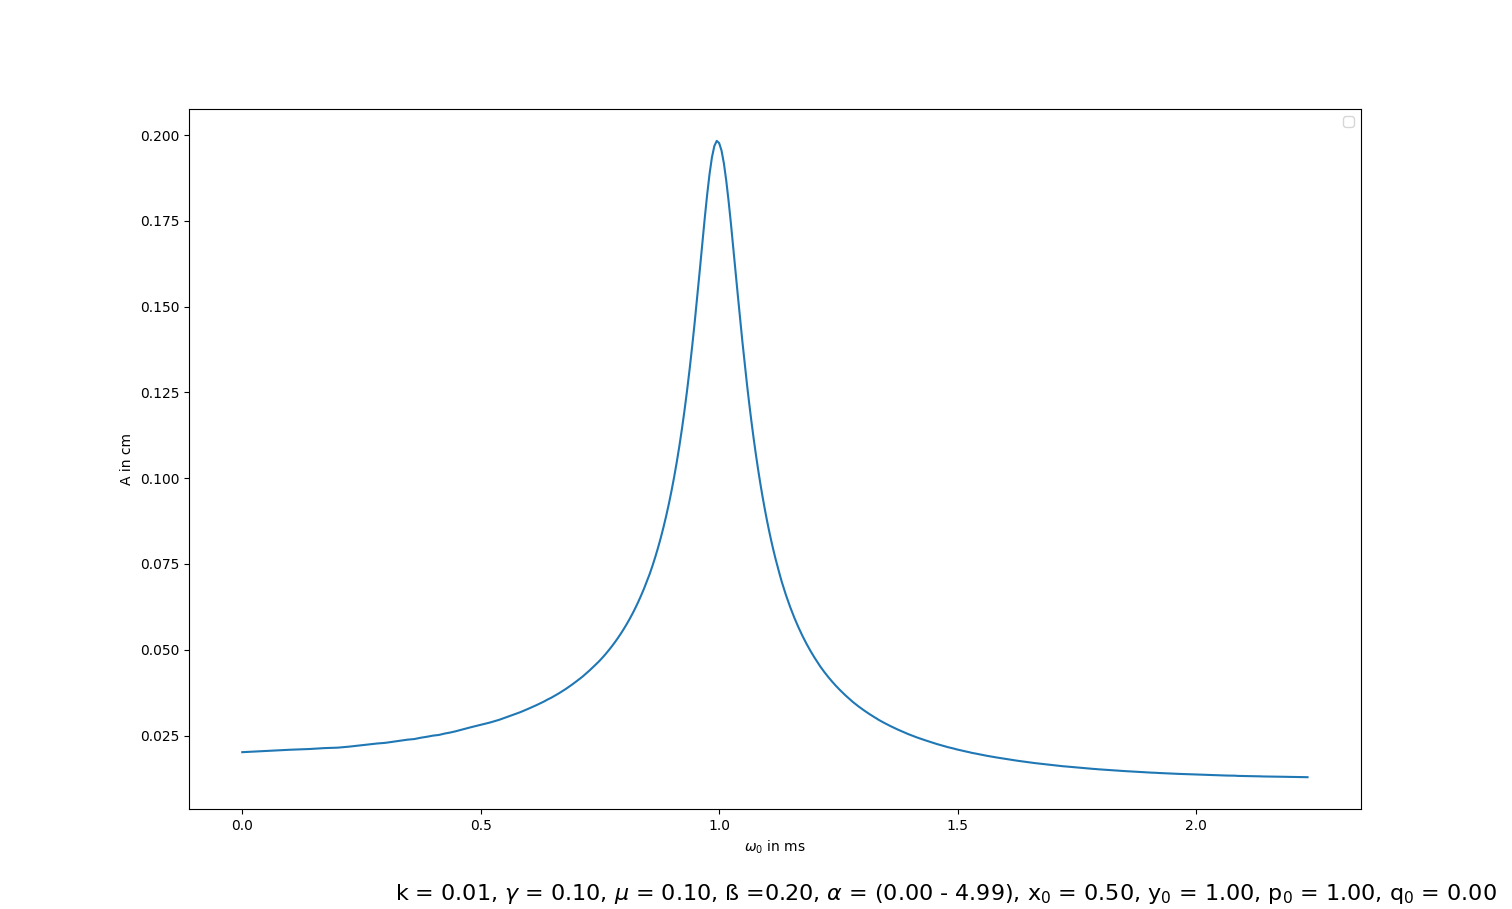
\includegraphics[width=\textwidth]{resonanz2.png}
			\caption{}
			\label{fig:resonanz2}
		\end{subfigure}
		\begin{subfigure}[b]{0.45\textwidth}
			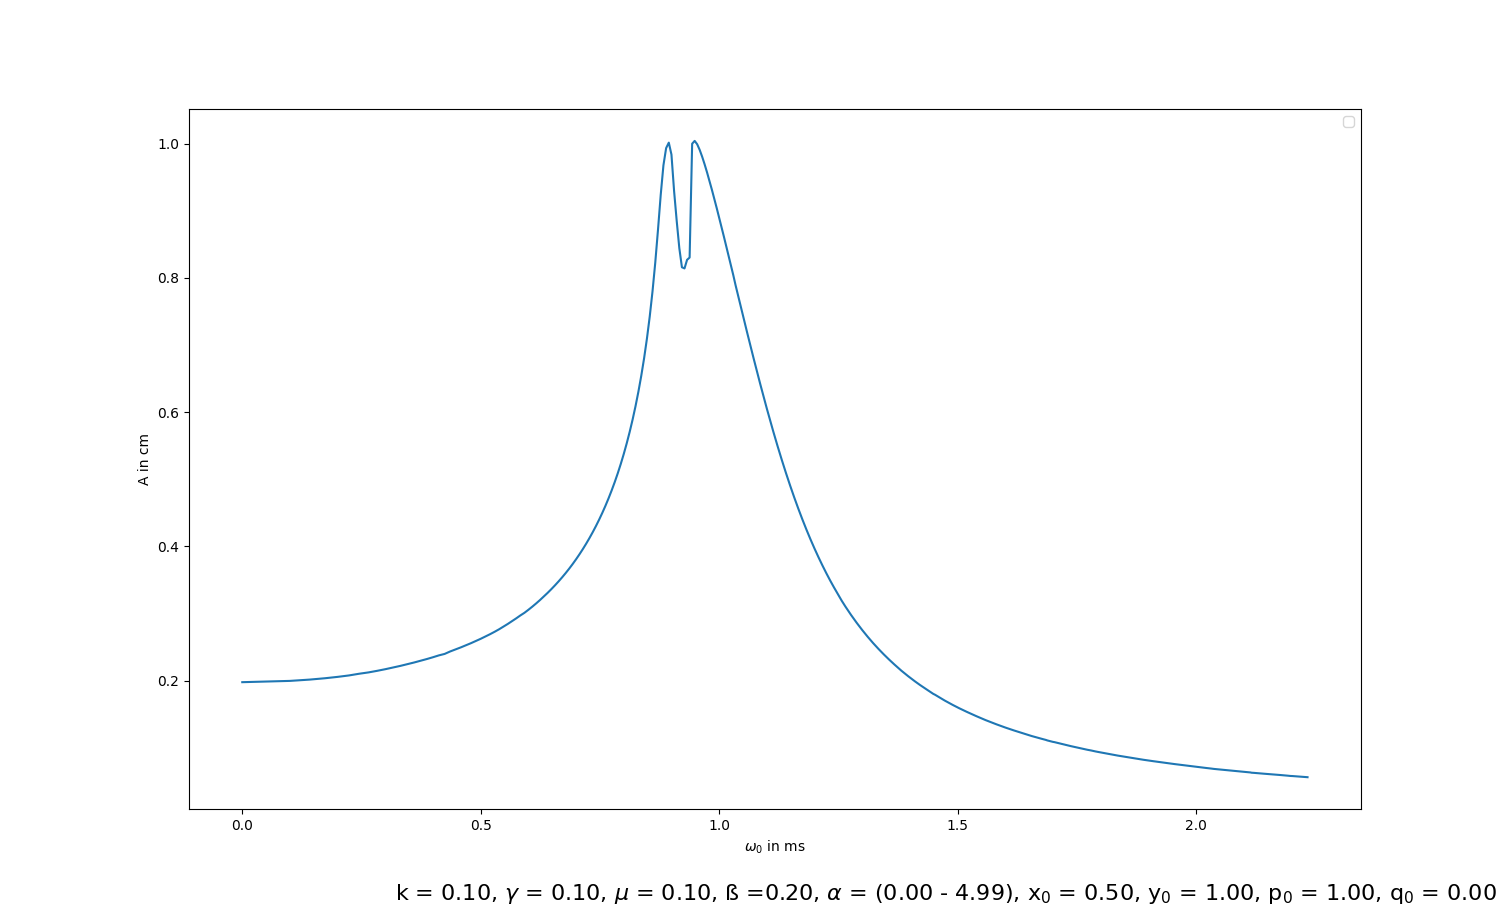
\includegraphics[width=\textwidth]{resonanz3.png}
			\caption{}
			\label{fig:resonanz3}
		\end{subfigure}
		\hfill
		\begin{subfigure}[b]{0.45\textwidth}
			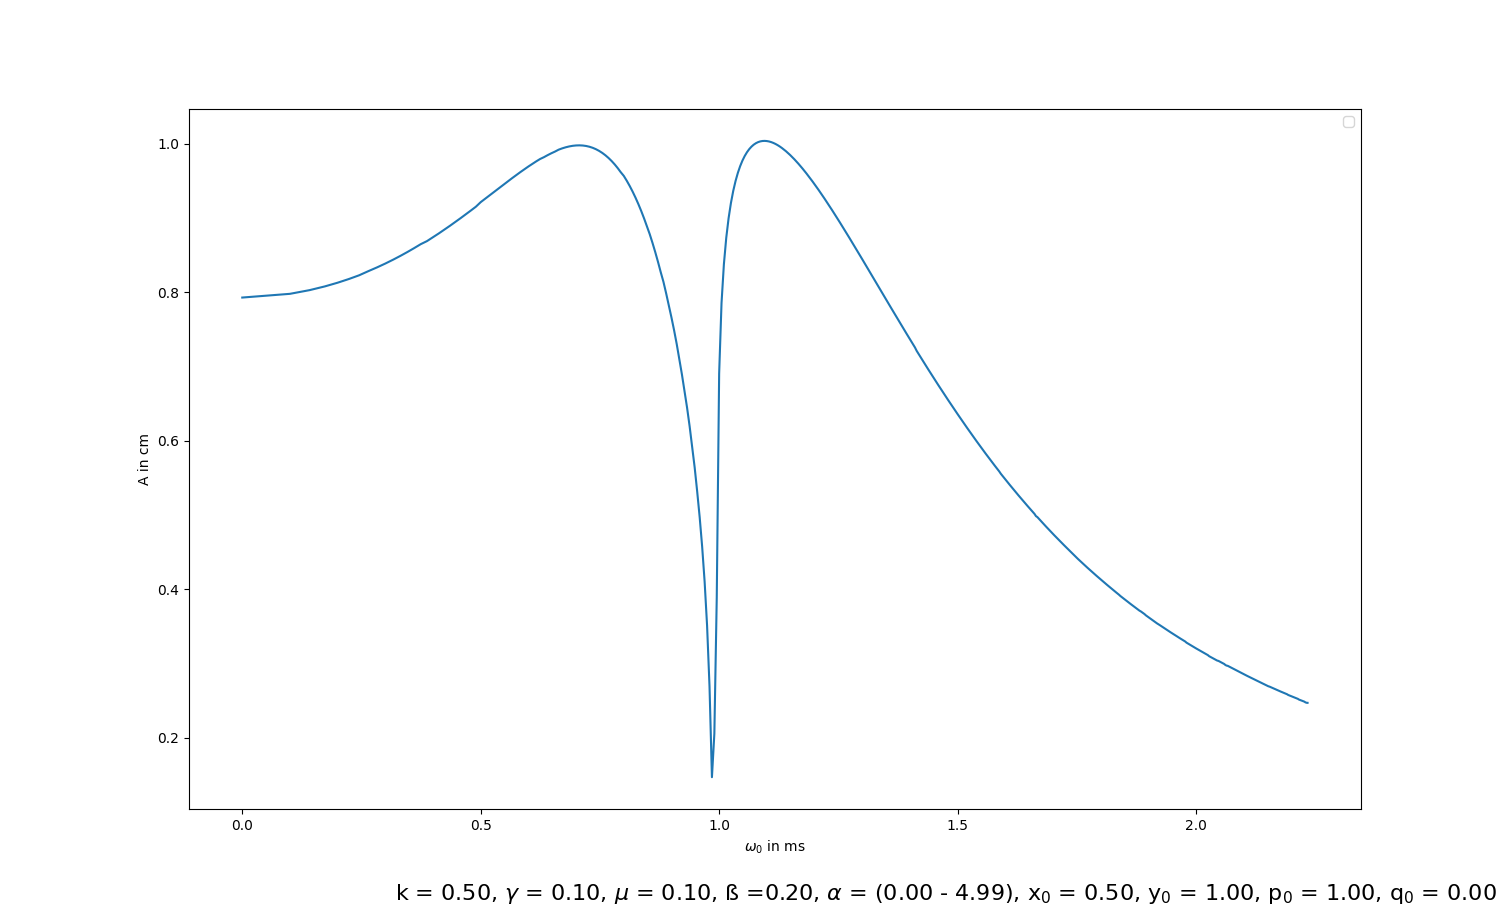
\includegraphics[width=\textwidth]{resonanz4.png}
			\caption{}
			\label{fig: resonanz4}
		\end{subfigure}
		\begin{subfigure}[b]{0.45\textwidth}
			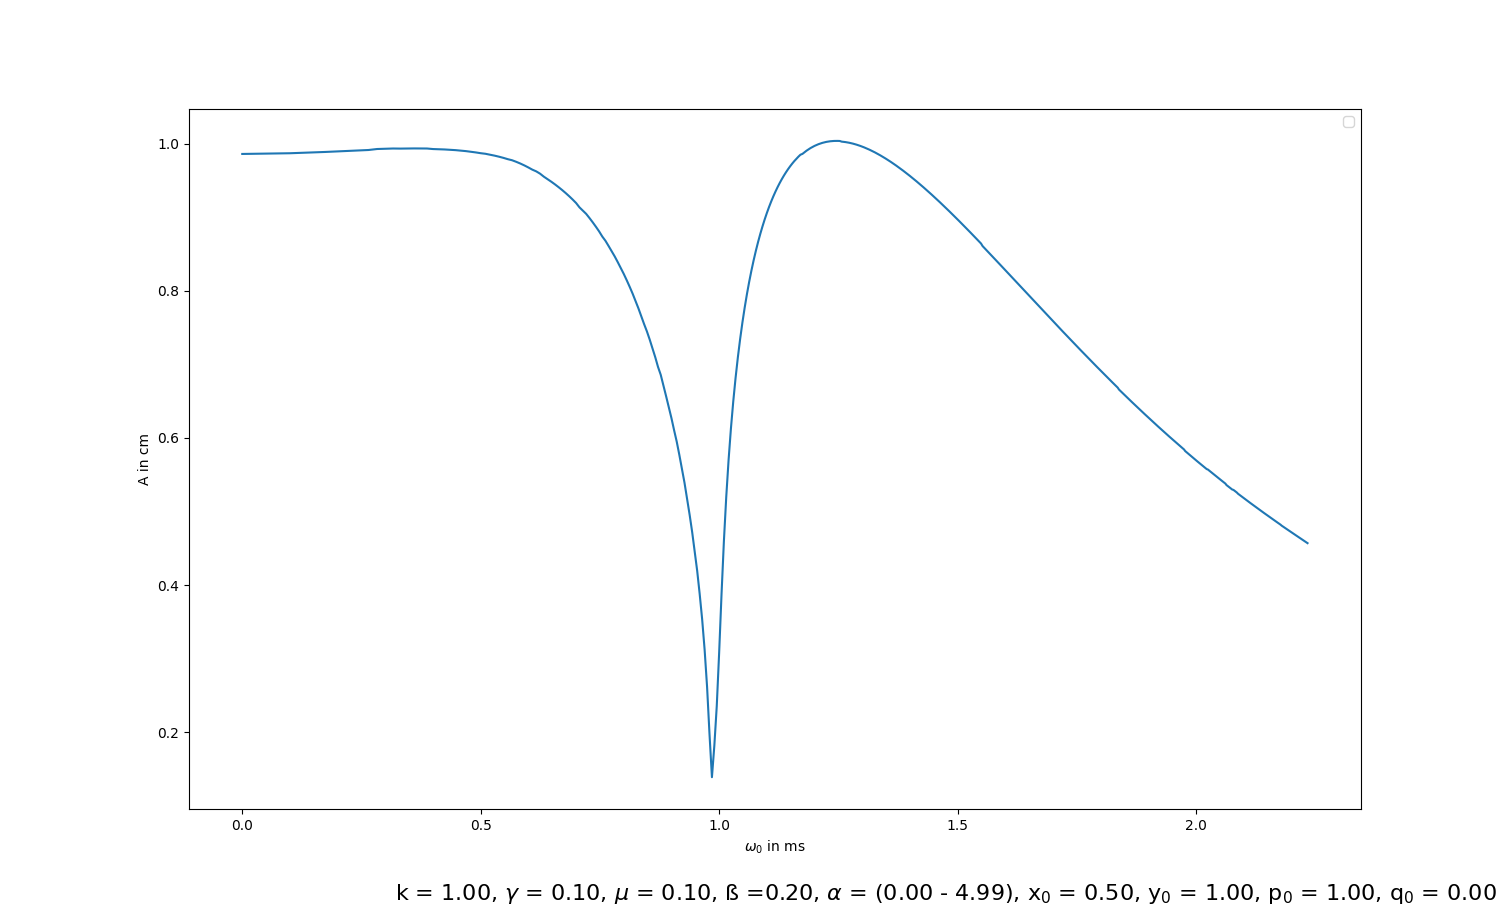
\includegraphics[width=\textwidth]{resonanz5.png}
			\caption{}
			\label{fig:resonanz5}
		\end{subfigure}
		
		\caption{Amplitude response of Duffing - Oscillator driven by Van der Pol - Oscillator. The Couplingconstant k are 0.00, 0.01, 0.10, 0.50 and 1.00 for the giving Parameters: $\gamma$ = 0.1, $\alpha$ = (0.00 - 5.00) and $\beta$ = 0.2, $\mu$ = 0.1. The giving Startingpoint for this simulation is (x, q, y,p) = (0.5, 0.0, 1.0, 1.0).}
		\label{fig:resonanz}
	\end{figure}
		
		
	\chapter{Outlook}	
		Die Klangerzeugung mittels Stimmlippen ist ein nichtlineares Verhalten. Ein geeignetes Modell zu bauen, hilft, um zu verstehen wie Frequenzen, Formanten und Obertöne entstehen.
		Wie erzeugt es Daniel Priegnitz die Schreigesänge mittels seine Falschen Stimmlippen und findet man in diesen Model bifurkationsmuster?
		Wie verhält sich das System wenn die Kopplungskonstante k > 1 ist? 
	\addcontentsline{toc}{chapter}{Bibliography}
	\bibliographystyle{plainurl}
	\nocite{*}
	\bibliography{Literatur}
	\newpage
\end{document}